\documentclass[10pt]{article}
\usepackage[utf8]{inputenc}
\usepackage{parskip}
\usepackage[margin = 1in]{geometry}
\usepackage{xcolor}
\usepackage[colorlinks = true,linkcolor = blue, urlcolor  = blue,citecolor = blue,anchorcolor = blue]{hyperref}
\usepackage{framed}
\usepackage{apacite}
\usepackage[authoryear,sort]{natbib}
\usepackage{amsmath}
\bibliographystyle{apalike}
\newcommand{\E}{\textrm{E}}
\renewcommand*{\theenumi}{\thesection.\arabic{enumi}}
\renewcommand{\P}{\text{P}}
\usepackage{tikz}
\usetikzlibrary{arrows,shapes.arrows,positioning,shapes,patterns,calc}

\begin{document}

\begin{Large} 
Info 6751. Fall 2022. Problem Set 4. Due on Canvas by 5pm on 19 Sep.
\end{Large}
\hline

This is our first problem set involving analysis of data. This first page provides the context for the data we will use. The second page contains the problem set.

In an influential paper, \href{https://www.jstor.org/stable/1806062}{LaLonde (1986)} argued that observational studies can produce misleading causal claims. LaLonde used two data sources to make this argument: (1) an experiment where people were randomized to a control condition or a job training condition and (2) observational data on people who did not receive job training. The first data source provided an experimental benchmark estimate. To make a non-experimental comparison, LaLonde took the treated units from (1), pooled them with the untreated units from (2), and then used econometric methods for causal inference.

Side note: The LaLonde study is influential, but it is also complicated. To me, it is not entirely clear that the experimentally-treated and observationally-control observations come from the same target population, for instance. We will set aside these concerns and work with the data anyhow.

In a reanalysis, Dehejia \& Wahba (\href{https://www.tandfonline.com/doi/abs/10.1080/01621459.1999.10473858}{1999}, \href{https://doi.org/10.1162/003465302317331982}{2002}) used a new set of methods and were more successful at recovering the experimental benchmark. We will cover those methods later in the semester. For today, we will use the data provided by Dehejia \& Wahba. The original link is \href{https://users.nber.org/~rdehejia/nswdata2.html}{here}, but I prepared a simpler version of the data. You should download \texttt{lalonde.csv} from the assignment page on the course website.

The file \texttt{lalonde.csv} contains 313 observations on 6 variables.
\begin{itemize}
    \item treated: 0 for untreated (no job training), 1 for treated (job training)
    \item y: 0/1 indicator coded one if earnings in 1978 are greater than 0
    \item race: categorical variable coded (Black, Hispanic, other)
    \item married: 0/1 indicator coded 1 if the respondent is married
    \item nodegree: 0/1 indicator coded 1 if the respondent did not finish high school
    \item education: years of schooling (numeric)
\end{itemize}

Throughout the problem, we will assume this DAG.

\begin{center}
    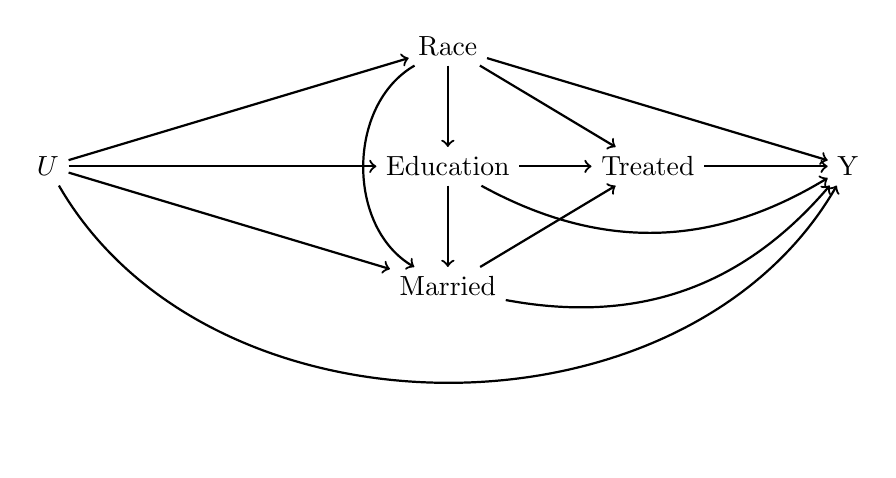
\begin{tikzpicture}[x = 1in, y = .6in]
        \node (r) at (0,1) {Race};
        \node (e) at (0,0) {Education};
        \node (m) at (0,-1) {Married};
        \node (a) at (1,0) {Treated};
        \node (y) at (2,0) {Y};
        \node (u) at (-2,0) {$U$};
        \draw[->, thick] (r) -- (e);
        \draw[->, thick] (e) -- (m);
        \draw[->, thick] (r) to[bend right = 60] (m);
        \draw[->, thick] (r) -- (y);
        \draw[->, thick] (e) to[bend right] (y);
        \draw[->, thick] (m) to[bend right] (y);
        \draw[->, thick] (u) -- (r);
        \draw[->, thick] (u) -- (e);
        \draw[->, thick] (u) -- (m);
        \draw[->, thick] (u) to[bend right = 60] (y);
        \draw[->, thick] (r) -- (a);
        \draw[->, thick] (e) -- (a);
        \draw[->, thick] (m) -- (a);
        \draw[->, thick] (a) -- (y);
    \end{tikzpicture}
\end{center}
Importantly, in one part we will operationalize ``Education'' as the binary \texttt{nodegree} variable. In another part, we will operationalize ``Education'' as the numeric \texttt{education} variable, operationalized as a categorical predictor.

\clearpage

\section{(30 points) Material covered Tuesday}
Part 1 is about the \textbf{positivity}.

Recall from class that for a treatment $A$ and a set of confounders $\vec{X}$, positivity is the assumption that $\P(A = a\mid \vec{X} = \vec{x}) > 0$ for all $a$ and $\vec{x}$. The assumption guarantees that in an infinite sample, we would observe an infinite set of people at every treatment value $a$ within every covariate stratum $\vec{x}$.

A second version of the positivity assumption is more empirical: in my sample, do I have every treatment value $a$ represented within each covariate stratum $\vec{x}$? This problem set deals with empirical positivity.

For 1.1 and 1.2, let the confounder set be \{\texttt{race}, \texttt{married}, \texttt{nodegree}\}.
\begin{enumerate}
    \item (5 points) Does empirical positivity hold in our sample?
    \item (10 points) With the confounder set from (1.1), nonparametrically estimate the sample average treatment effect. Specifically: (1) estimate the treatment effect within each subgroup and (2) aggregate over subgroups, weighted by the number of units in each subgroup. Interpret your answer in a sentence with units.
\end{enumerate}
Suppose we now believe that \texttt{nodegree} is an unacceptably coarse measure of education: years of education confounds treatment assignment within levels of \texttt{nodegree}. For the remainder of this problem set, take \{\texttt{race}, \texttt{married}, \texttt{nodegree}\} to be the confounder set.
\begin{enumerate}\setcounter{enumi}{2}
    \item (5 points) For what proportion of the sample does empirical positivity hold? In other words, what proportion of the sample resides in a covariate stratum where both treated and control units are observed?
    \item (10 points) Because the answer to 1.3 is less than 100\%, nonparametric estimation for the full sample is impossible. Instead, restrict to the covariate strata for which empirical positivity holds. Nonparametrically estimate the average causal effect in this feasible subsample.
\end{enumerate}

\section{(20 points) Material covered Thursday}
Part 2 is about the \textbf{parametric $g$-formula}. When empirical positivity does not hold and we want to estimate the average treatment effect in the full sample, we must rely on parametric assumptions.
\begin{enumerate}
    \item (20 points) Assume an Ordinary Least Squares specification including these predictors:
\begin{itemize}
    \item the treatment
    \item race
    \item marital status
    \item the interaction between treatment and race
    \item the interaction between treatment and marital status
    \item years of education, entered as a categorical predictor, not interacted with anything
\end{itemize}
Estimate the average treatment effect with this model, using the parametric $g$-formula. Specifically
\begin{itemize}
    \item Fit the outcome model.
    \item Change everyone's treatment to 1. Predict each outcome $Y_i^1$.
    \item Change everyone's treatment to 0. Predict each outcome $Y_i^0$.
    \item Take the difference for every person: $Y_i^1 - Y_i^0$.
    \item Average over the sample to produce an estimate.
\end{itemize}
\end{enumerate}

\end{document}

